\documentclass[11pt,a4paper]{article}

\usepackage[a4paper,margin=1in]{geometry}
\usepackage[T1]{fontenc}
\usepackage[utf8]{inputenc}
\usepackage{lmodern}
\usepackage{microtype}
\usepackage{amsmath,amssymb}
\usepackage{booktabs}
\usepackage{array}
\usepackage{tabularx}
\usepackage{longtable}
\usepackage{graphicx}
\usepackage{xcolor}
\usepackage{tikz}
\usetikzlibrary{arrows.meta,positioning,fit,calc,shapes.geometric,3d,perspective}
\usepackage{listings}
\usepackage{enumitem}
\usepackage{float}
\usepackage{caption}
\usepackage{subcaption}
\usepackage{hyperref}
\usepackage{fancyhdr}
\usepackage{lastpage}
\usepackage{titlesec}
\usepackage{setspace}

\definecolor{iitblue}{HTML}{143D59}
\definecolor{iitgold}{HTML}{F4B942}
\definecolor{lightblue}{HTML}{EAF2F8}
\definecolor{lightgray}{HTML}{F4F5F7}
\definecolor{darkgray}{HTML}{404040}
\definecolor{midblue}{HTML}{3975A5}
\definecolor{palegold}{HTML}{FFF4D6}
\definecolor{palegreen}{HTML}{E8F4EE}

\hypersetup{
  colorlinks=true,
  linkcolor=iitblue,
  urlcolor=iitblue,
  citecolor=iitblue,
  pdftitle={IIT Jodhpur Academic Helpdesk},
  pdfauthor={Mohi1038 Academic Helpdesk Team}
}

\pagestyle{fancy}
\fancyhf{}
\lhead{\small IIT Jodhpur Academic Helpdesk}
\rhead{\small Project Report}
\cfoot{\small\thepage\ of \pageref{LastPage}}
\setlength{\headheight}{14pt}
\setlength{\parskip}{3pt}
\setlength{\parindent}{0pt}
\setlist{itemsep=2pt,topsep=4pt}
\titleformat{\section}{\Large\bfseries\color{iitblue}}{\thesection}{0.7em}{}
\titleformat{\subsection}{\large\bfseries\color{iitblue}}{\thesubsection}{0.7em}{}
\titleformat{\subsubsection}{\normalsize\bfseries\color{darkgray}}{\thesubsubsection}{0.7em}{}

\lstset{
  basicstyle=\ttfamily\small,
  backgroundcolor=\color{lightgray},
  frame=single,
  rulecolor=\color{gray!40},
  breaklines=true,
  columns=fullflexible,
  showstringspaces=false
}

\newcommand{\systemname}{Academic Helpdesk Agent}
\newcommand{\tool}[1]{\texttt{#1}}
\newcommand{\metric}[1]{\textbf{#1}}

\begin{document}

\begin{titlepage}
\centering
\vspace*{1cm}
{\Large\textsc{Indian Institute of Technology Jodhpur}\par}
\vspace{0.4cm}
{\large Academic Helpdesk Agent\par}
\vspace{1.3cm}
{\Huge\bfseries Design, Implementation and Evaluation of a\\[0.2cm]
Multi-Agent Academic Helpdesk\par}
\vspace{1.0cm}

\begin{tikzpicture}
  \draw[fill=iitblue!8,draw=iitblue,line width=1pt,rounded corners=5pt]
    (0,0) rectangle (11,2.1);
  \node[align=center,text width=9.8cm] at (5.5,1.05)
    {\large A grounded question-answering and email-drafting system\\
     using Google ADK, Ollama-hosted language models, ChromaDB and hybrid RAG};
\end{tikzpicture}
\vfill
\begin{tabular}{ll}
\textbf{Team member} & \textbf{Roll number}\\
\midrule
Mohit Meemraauth & B23CS1038\\
Nisarg Upadhyay & B23CS1075\\
Divyansh Maheshwari & B23CM1015\\
Tejas Kalkar & B23CM1051\\
\end{tabular}
\vfill
{\large Project Report\par}
{\large Academic Year 2026--27\par}
\end{titlepage}

\pagenumbering{roman}
\begin{abstract}
This report presents the design and evaluation of a local, multi-agent Academic Helpdesk for IIT Jodhpur. The system answers questions about academic regulations, curricula, course offerings and timetables; drafts (but never sends) emails to course instructors; and refuses and logs questions outside its verified knowledge domain. The implementation combines Google Agent Development Kit (ADK), Ollama-hosted 8B language models, ChromaDB, local embeddings and a hybrid dense--BM25 retrieval pipeline. The corpus contains 29 public IIT Jodhpur documents and structured data files for courses, timetable slots, faculty contacts and a student profile. 

The evaluation contains 30 questions, three model families, single-agent and multi-agent configurations, and three repeated runs per configuration, producing 630 graded answers. Qwen3:8b is the strongest overall model: the single-agent configuration reaches 80.6\% in-scope accuracy, while the multi-agent configuration reaches 79.9\% with 94\% grounded answers and 100\% correct out-of-scope refusals. The multi-agent design improves routing and policy performance, but the thinking-enabled orchestrator increases mean latency from 10.9\,s to 30.0\,s. The results show that reliable tools, explicit citation requirements, deterministic refusal logging and directory-validated email drafting are as important as model choice.
\end{abstract}

\noindent\textbf{Keywords:} academic helpdesk, multi-agent systems, retrieval-augmented generation, Google ADK, Ollama, ChromaDB, grounded question answering

\tableofcontents
\clearpage
\pagenumbering{arabic}

\section{Introduction}
\label{sec:introduction}

Students regularly need small but consequential academic facts: the attendance rule for an examination, the meeting time of a course, the number of credits required for graduation, or the correct authority to whom a leave application should be addressed. These facts are distributed across regulations, circulars, curriculum documents, calendars, timetable sheets and faculty directories. A general-purpose chatbot can answer fluently while silently mixing old and new rules, inventing a timetable, or hallucinating an instructor's email address.

The objective of this project is therefore not simply to build a conversational interface. It is to build a bounded academic information system that:
\begin{enumerate}[leftmargin=*]
  \item answers questions only when evidence is available in an institutional corpus or an approved structured data source;
  \item cites the source used for the answer;
  \item routes questions to specialists for policy, schedule and email tasks;
  \item refuses and logs out-of-scope questions instead of guessing;
  \item drafts emails for student review without sending them; and
  \item remains executable on a laptop with approximately 16\,GB RAM using local models.
\end{enumerate}

The rest of this report describes the corpus, architecture, retrieval and agent design, evaluation methodology, quantitative results, observed failure modes and recommendations for a production-quality deployment.

\section{Requirements and Scope}
\label{sec:requirements}

\subsection{In-scope capabilities}
The helpdesk supports four functional categories:
\begin{itemize}[leftmargin=*]
  \item \textbf{Policy and curriculum:} academic regulations, attendance, examination rules, degree credits, add/drop dates and academic calendars.
  \item \textbf{Schedule:} course lookup, slot and room lookup, student timetable queries and counting courses by department, level or semester.
  \item \textbf{Email assistance:} instructor contact lookup and drafting of leave or make-up examination emails.
  \item \textbf{Safety and escalation:} refusal of unsupported questions and persistent logging for staff follow-up.
\end{itemize}

\subsection{Out-of-scope behavior}
Questions about dining options, travel directions, campus facilities, placement statistics or other topics not represented in the corpus must receive a refusal rather than an inferred answer. A refusal is treated as a successful behavior when the question is genuinely outside the verified domain. It must also be logged in \texttt{logs/unanswered.jsonl}.

\subsection{Representative questions}
\begin{table}[H]
\centering
\caption{Representative questions covered by the system.}
\label{tab:representative}
\small
\begin{tabularx}{\textwidth}{>{\raggedright\arraybackslash}p{0.25\textwidth}X}
\toprule
\textbf{Category} & \textbf{Example}\\
\midrule
Policy & What is the attendance requirement to sit in the Major exam?\\
Schedule & What is the slot for the course Autonomous Systems?\\
Counting & How many 400-level electives have been floated by the Humanities department this semester?\\
Degree & How many Open Elective credits are required for a B.Tech. degree?\\
Email & Write an email to the instructor of CSL7570 that I need leave for two days.\\
Out of scope & What are the available dining options on campus?\\
\bottomrule
\end{tabularx}
\end{table}

\section{Data Collection and Knowledge Sources}
\label{sec:data}

\subsection{Document corpus}
The project collected 29 public IIT Jodhpur sources: 24 PDFs and five web pages. The sources cover academic regulations, attendance and examination amendments, academic calendars, holidays, fees, scholarships, medical forms, B.Tech./M.Tech. curricula, common courses, non-graded courses and humanities courses. The manifest records document title, category, source URL, fetch date, page count and a content hash.

\begin{table}[H]
\centering
\caption{Knowledge sources used by the helpdesk.}
\label{tab:corpus}
\small
\begin{tabularx}{\textwidth}{>{\raggedright\arraybackslash}p{0.25\textwidth} >{\centering\arraybackslash}p{0.14\textwidth} X}
\toprule
\textbf{Source type} & \textbf{Count} & \textbf{Examples and role}\\
\midrule
PDF documents & 24 & Regulations, curricula, circulars, calendars, fees, scholarships and forms.\\
Web pages & 5 & Academic programmes, registration, engineering/science information and contact pages.\\
Structured CSV/JSON & 4 & Course offerings, timetable, faculty directory and student profile.\\
\midrule
\textbf{Total public documents} & \textbf{29} & Indexed for retrieval and citation.\\
\bottomrule
\end{tabularx}
\end{table}

\subsection{Structured data and data quality}
Structured lookup tools complement document retrieval. The course catalogue describes Semester I of AY 2026--27, the official slot system stores standard meeting times, the faculty directory supplies instructor contacts, and the student profile enables questions such as ``What classes do I have on Friday?'' Course titles, levels, credits and several faculty facts are sourced from IIT Jodhpur material. Course codes not published by the source documents, course-to-instructor assignments and some slot/room mappings are explicitly marked illustrative or synthetic in the repository documentation. This distinction prevents synthetic test data from being mistaken for official institutional policy.

\section{System Architecture}
\label{sec:architecture}

\subsection{High-level architecture}
The final system has two modes. The baseline is a single ADK \texttt{LlmAgent} with all tools. The proposed multi-agent mode uses an orchestrator with no domain tools; it transfers each request to a policy, schedule or email specialist. The same retrieval and structured tools are used in both modes.

\begin{figure}[H]
\centering
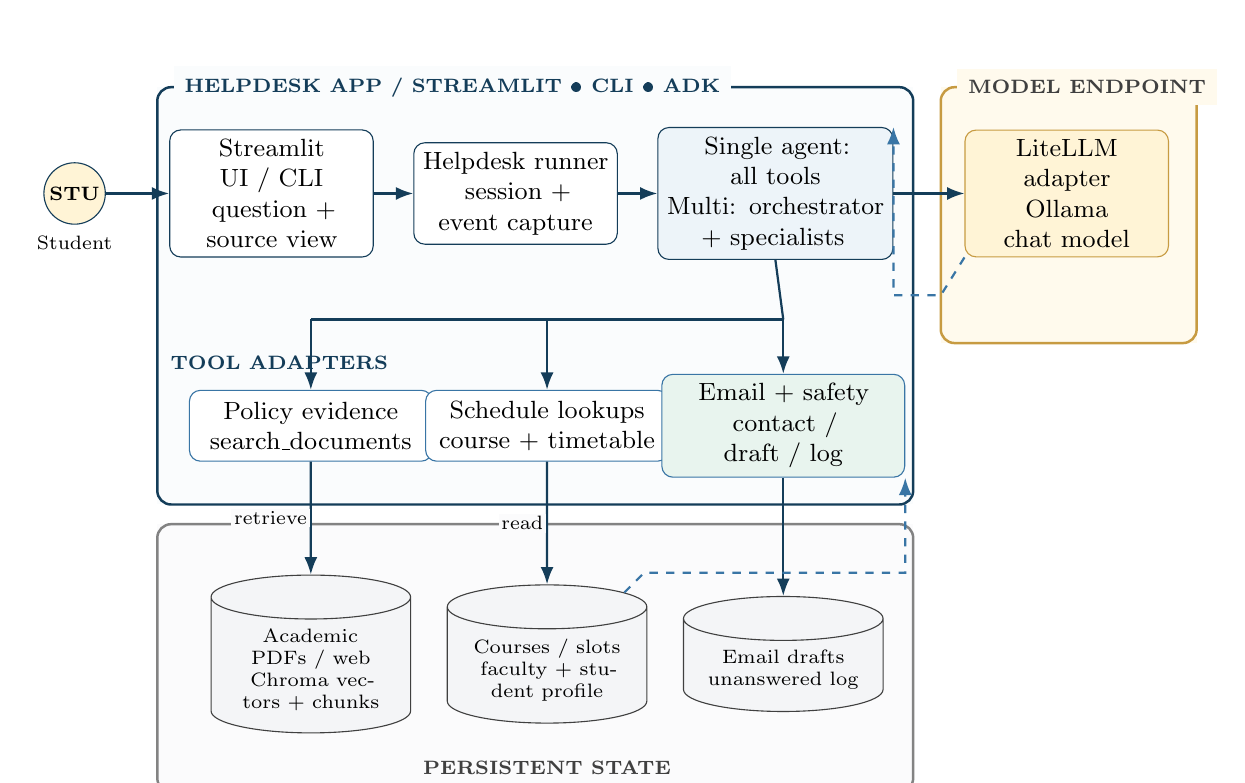
\begin{tikzpicture}[
  panel/.style={rounded corners=5pt,line width=0.9pt},
  component/.style={draw=iitblue,fill=white,rounded corners=4pt,
                    minimum height=0.9cm,text width=2.35cm,align=center,font=\small},
  agent/.style={component,draw=iitblue,fill=lightblue!85,text width=2.75cm},
  tool/.style={component,draw=midblue,fill=white,text width=2.85cm},
  store/.style={cylinder,shape border rotate=90,aspect=0.22,draw=darkgray,
                fill=lightgray,minimum height=1.05cm,text width=2.3cm,
                align=center,font=\scriptsize},
  arr/.style={-{Latex[length=2.2mm]},thick,draw=iitblue},
  ret/.style={-{Latex[length=2.2mm]},thick,dashed,draw=midblue}
]
  % Context boundaries
  \fill[lightblue!22] (1.05,3.3) rectangle (10.65,-2.0);
  \draw[panel,draw=iitblue] (1.05,3.3) rectangle (10.65,-2.0);
  \node[anchor=west,font=\scriptsize\bfseries,color=iitblue,fill=lightblue!22,inner sep=4pt]
    at (1.25,3.3) {HELPDESK APP  /  STREAMLIT • CLI • ADK};
  \fill[palegold!45] (11.0,3.3) rectangle (14.25,0.05);
  \draw[panel,draw=iitgold!75!darkgray] (11.0,3.3) rectangle (14.25,0.05);
  \node[anchor=west,font=\scriptsize\bfseries,color=darkgray,fill=palegold!45,inner sep=4pt]
    at (11.2,3.3) {MODEL ENDPOINT};
  \fill[lightgray!40] (1.05,-2.25) rectangle (10.65,-5.65);
  \draw[panel,draw=darkgray!65] (1.05,-2.25) rectangle (10.65,-5.65);

  % Request and inference path
  \node[circle,draw=iitblue,fill=palegold,minimum size=0.78cm,inner sep=1pt,
        font=\scriptsize\bfseries] (student) at (0,1.95) {STU};
  \node[font=\scriptsize] at (0,1.33) {Student};
  \node[component] (ui) at (2.5,1.95) {Streamlit UI / CLI\\question + source view};
  \node[component] (runner) at (5.6,1.95) {Helpdesk runner\\session + event capture};
  \node[agent] (agents) at (8.9,1.95) {Single agent: all tools\\Multi: orchestrator + specialists};
  \node[component,draw=iitgold!75!darkgray,fill=palegold,text width=2.35cm] (ollama) at (12.6,1.95)
    {LiteLLM adapter\\Ollama chat model};
  \draw[arr] (student) -- (ui);
  \draw[arr] (ui) -- (runner);
  \draw[arr] (runner) -- (agents);
  \draw[arr] (agents.east) -- (ollama.west);
  \draw[ret] (ollama.south west) -- ++(-0.3,-0.48) -| (agents.north east);

  % Tool adapters: grouped by the data they are allowed to use
  \node[font=\scriptsize\bfseries,color=iitblue] at (2.6,-0.2) {TOOL ADAPTERS};
  \node[tool] (policy) at (3.0,-1.0) {Policy evidence\\search\_documents};
  \node[tool] (schedule) at (6.0,-1.0) {Schedule lookups\\course + timetable};
  \node[tool,fill=palegreen] (email) at (9.0,-1.0) {Email + safety\\contact / draft / log};
  \draw[thick,draw=iitblue] (agents.south) -- (9.0,0.35);
  \draw[thick,draw=iitblue] (3.0,0.35) -- (9.0,0.35);
  \draw[arr] (3.0,0.35) -- (policy.north);
  \draw[arr] (6.0,0.35) -- (schedule.north);
  \draw[arr] (9.0,0.35) -- (email.north);

  % Durable inputs and outputs
  \node[store] (documents) at (3.0,-4.1) {Academic PDFs / web\\Chroma vectors + chunks};
  \node[store] (catalogue) at (6.0,-4.1) {Courses / slots\\faculty + student profile};
  \node[store] (records) at (9.0,-4.1) {Email drafts\\unanswered log};
  \draw[arr] (policy.south) -- node[left,font=\scriptsize,fill=lightgray!40,inner sep=1pt]{retrieve} (documents.north);
  \draw[arr] (schedule.south) -- node[left,font=\scriptsize,fill=lightgray!40,inner sep=1pt]{read} (catalogue.north);
  \draw[arr] (email.south) -- ++(0,-0.45) -| (records.north);
  \draw[ret] (catalogue.north east) -- ++(0.25,0.25) -| (email.south east);
  \node[font=\scriptsize\bfseries,color=darkgray] at (6.0,-5.35) {PERSISTENT STATE};
\end{tikzpicture}
\caption{Runtime architecture and trust boundaries. The application contains the interface, runner, agent mode and tool adapters. Ollama serves model inference separately; the retriever, structured catalogues and generated files form distinct data paths.}
\label{fig:architecture}
\end{figure}

\subsection{Agent responsibilities}
\begin{table}[H]
\centering
\caption{Agents and allowed responsibilities.}
\label{tab:agents}
\small
\begin{tabularx}{\textwidth}{>{\bfseries}p{0.28\textwidth} X}
\toprule
Agent & Responsibility and tools\\
\midrule
Helpdesk orchestrator & Understands the request, transfers to one specialist, and refuses/logs unsupported topics.\\
Policy agent & Searches regulations, curricula, circulars and calendars using \tool{search\_documents}.\\
Schedule agent & Uses \tool{find\_course}, \tool{list\_courses}, \tool{get\_slot\_timetable} and \tool{get\_my\_schedule}.\\
Email agent & Uses \tool{get\_instructor\_contact} and \tool{draft\_email}; it never sends messages.\\
Safety callback & An \texttt{after\_agent\_callback} logs refusals that the model fails to log explicitly.\\
\bottomrule
\end{tabularx}
\end{table}

\clearpage
\begin{figure}[H]
\centering
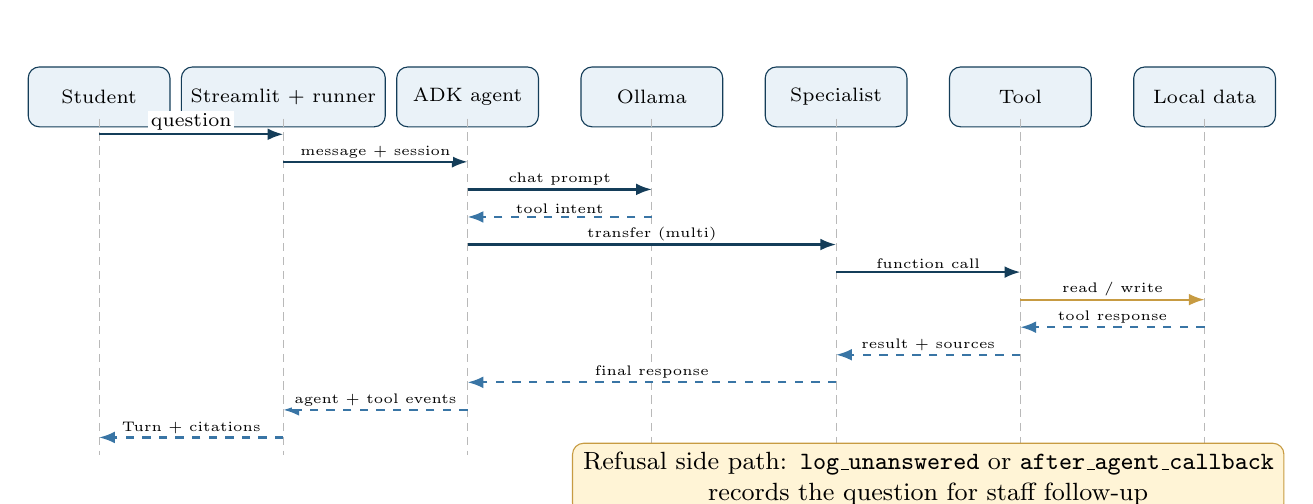
\begin{tikzpicture}[x=0.78cm,y=0.50cm,>=Latex,
  participant/.style={draw=iitblue,fill=lightblue,rounded corners=4pt,
                     minimum width=1.8cm,minimum height=0.76cm,align=center,font=\scriptsize},
  lifeline/.style={draw=gray!55,densely dashed},
  call/.style={-{Latex[length=2mm]},thick,draw=iitblue},
  response/.style={-{Latex[length=2mm]},thick,dashed,draw=midblue},
  persistence/.style={-{Latex[length=2mm]},thick,draw=iitgold!75!darkgray}
]
  \foreach \x/\name in {0/Student,3/Streamlit + runner,6/ADK agent,9/Ollama,12/Specialist,15/Tool,18/Local data} {
    \node[participant] at (\x,0) {\name};
    \draw[lifeline] (\x,-0.55) -- (\x,-9.1);
  }
  \draw[call] (0,-0.95) -- node[above,font=\scriptsize,fill=white,inner sep=1pt]{question} (3,-0.95);
  \draw[call] (3,-1.65) -- node[above,font=\tiny,fill=white,inner sep=1pt]{message + session} (6,-1.65);
  \draw[call] (6,-2.35) -- node[above,font=\tiny,fill=white,inner sep=1pt]{chat prompt} (9,-2.35);
  \draw[response] (9,-3.05) -- node[above,font=\tiny,fill=white,inner sep=1pt]{tool intent} (6,-3.05);
  \draw[call] (6,-3.75) -- node[above,font=\tiny,fill=white,inner sep=1pt]{transfer (multi)} (12,-3.75);
  \draw[call] (12,-4.45) -- node[above,font=\tiny,fill=white,inner sep=1pt]{function call} (15,-4.45);
  \draw[persistence] (15,-5.15) -- node[above,font=\tiny,fill=white,inner sep=1pt]{read / write} (18,-5.15);
  \draw[response] (18,-5.85) -- node[above,font=\tiny,fill=white,inner sep=1pt]{tool response} (15,-5.85);
  \draw[response] (15,-6.55) -- node[above,font=\tiny,fill=white,inner sep=1pt]{result + sources} (12,-6.55);
  \draw[response] (12,-7.25) -- node[above,font=\tiny,fill=white,inner sep=1pt]{final response} (6,-7.25);
  \draw[response] (6,-7.95) -- node[above,font=\tiny,fill=white,inner sep=1pt]{agent + tool events} (3,-7.95);
  \draw[response] (3,-8.65) -- node[above,font=\tiny,fill=white,inner sep=1pt]{Turn + citations} (0,-8.65);
  \node[draw=iitgold!75!darkgray,fill=palegold,rounded corners=4pt,
        text width=8.8cm,align=center,font=\small] at (13.5,-9.7)
    {Refusal side path: \texttt{log\_unanswered} or \texttt{after\_agent\_callback} records the question for staff follow-up};
\end{tikzpicture}
\caption{Turn sequence through the runtime. Multi-agent mode adds the specialist transfer; single-agent mode calls the tools directly. In both modes, the runner captures agent and tool events before returning an answer, citations and any saved draft.}
\label{fig:sequence}
\end{figure}

\section{Retrieval-Augmented Generation Pipeline}
\label{sec:rag}

\subsection{Indexing}
PDF and web content is normalized, with scanned PDFs passed through OCR when necessary. Text is split into approximately 350-word, section-aware chunks. A one-paragraph overlap reduces boundary loss, while page ranges are retained for citations. Repeated headers and footers are removed before embedding.

\subsection{Hybrid retrieval}
Each query is processed by two complementary retrievers:
\begin{enumerate}[leftmargin=*]
  \item dense retrieval using the local \texttt{nomic-embed-text} model and ChromaDB; and
  \item lexical retrieval using BM25, which is particularly useful for exact course codes, clause numbers and dates.
\end{enumerate}
The ranked lists are fused with reciprocal rank fusion. A minimum dense similarity threshold is used as an early signal that a question may not be answerable from the corpus. The model prompt still has to verify that the returned passages answer the question.

\clearpage
\begin{figure}[H]
\centering
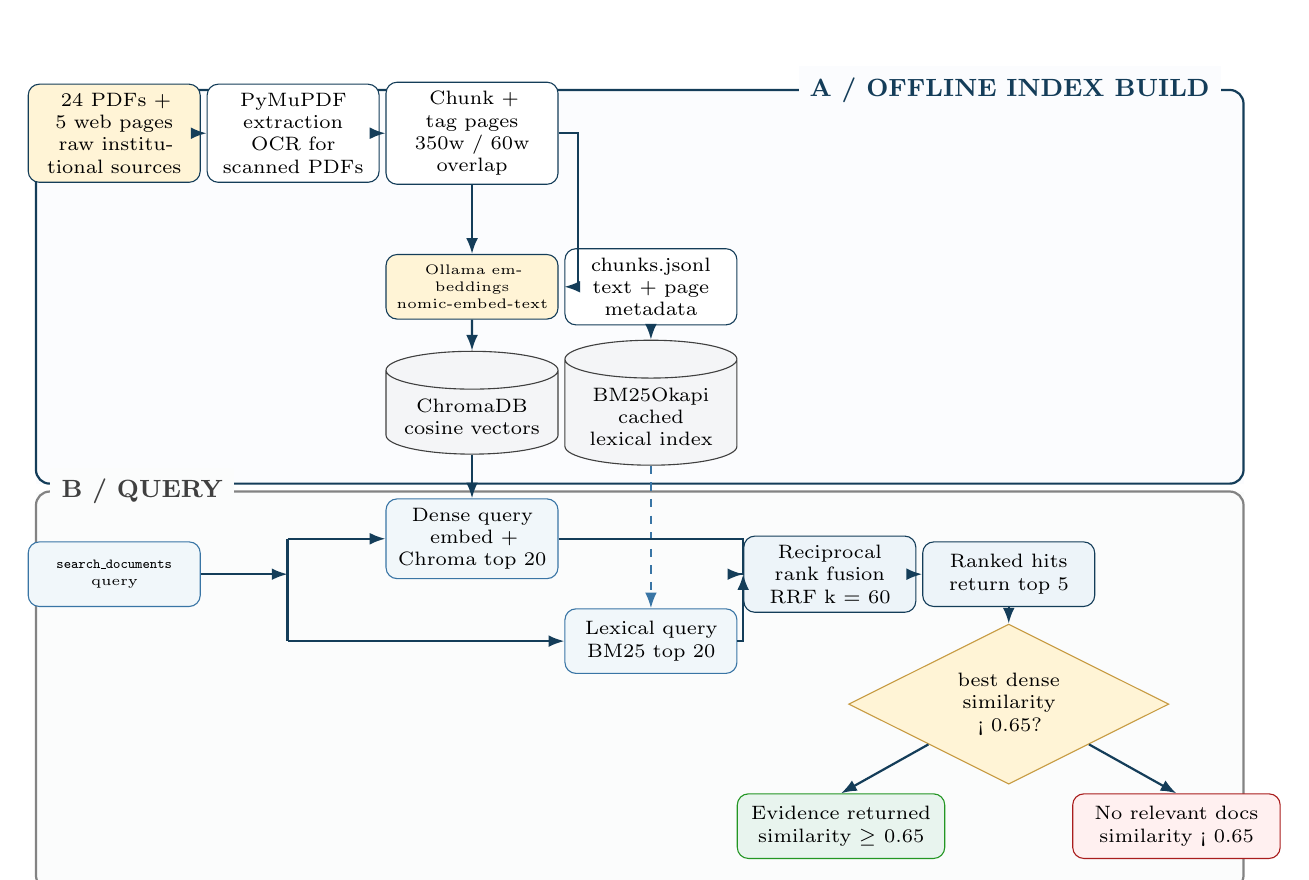
\begin{tikzpicture}[x=0.71cm,y=1.00cm,>=Latex,
  panel/.style={rounded corners=5pt,line width=0.8pt},
  process/.style={draw=iitblue,fill=white,rounded corners=4pt,
                  minimum height=0.82cm,text width=1.95cm,align=center,font=\scriptsize},
  index/.style={cylinder,shape border rotate=90,aspect=0.22,draw=darkgray,
                fill=lightgray,minimum height=0.92cm,text width=1.95cm,
                align=center,font=\scriptsize},
  query/.style={process,draw=midblue,fill=lightblue!65},
  fusion/.style={process,draw=iitblue,fill=lightblue!85},
  arr/.style={-{Latex[length=2mm]},thick,draw=iitblue},
  ret/.style={-{Latex[length=2mm]},thick,dashed,draw=midblue}
]
  % The upper frame is an offline build. The lower frame is query-time serving.
  \fill[lightblue!20] (-1.4,4.15) rectangle (20.2,-0.85);
  \draw[panel,draw=iitblue] (-1.4,4.15) rectangle (20.2,-0.85);
  \node[anchor=east,font=\small\bfseries,color=iitblue,fill=lightblue!20,inner sep=4pt]
    at (19.8,4.15) {A  /  OFFLINE INDEX BUILD};
  \fill[lightgray!32] (-1.4,-0.95) rectangle (20.2,-6.0);
  \draw[panel,draw=darkgray!65] (-1.4,-0.95) rectangle (20.2,-6.0);
  \node[anchor=west,font=\small\bfseries,color=darkgray,fill=lightgray!32,inner sep=4pt]
    at (-1.15,-0.95) {B  /  QUERY};

  % Index creation: one chunk stream feeds the semantic and lexical paths.
  \node[process,fill=palegold] (sources) at (0,3.6) {24 PDFs + 5 web pages\\raw institutional sources};
  \node[process] (extract) at (3.2,3.6) {PyMuPDF extraction\\OCR for scanned PDFs};
  \node[process] (chunker) at (6.4,3.6) {Chunk + tag pages\\350w / 60w overlap};
  \node[process,fill=palegold,font=\tiny] (embed) at (6.4,1.65) {Ollama embeddings\\nomic-embed-text};
  \node[index] (chroma) at (6.4,0.0) {ChromaDB\\cosine vectors};
  \node[process] (chunkfile) at (9.6,1.65) {chunks.jsonl\\text + page metadata};
  \node[index] (bmindex) at (9.6,0.0) {BM25Okapi\\cached lexical index};
  \draw[arr] (sources.east) -- (extract.west);
  \draw[arr] (extract.east) -- (chunker.west);
  \draw[arr] (chunker.south) -- (embed.north);
  \draw[arr] (embed.south) -- (chroma.north);
  \draw[arr] (chunker.east) -- ++(0.35,0) |- (chunkfile.west);
  \draw[arr] (chunkfile.south) -- (bmindex.north);

  % Two query paths read their matching indexes, then merge by rank.
  \node[query,font=\tiny] (search) at (0,-2.0) {\texttt{search\_documents}\\query};
  \node[query] (denseq) at (6.4,-1.55) {Dense query\\embed + Chroma top 20};
  \node[query] (lexq) at (9.6,-2.85) {Lexical query\\BM25 top 20};
  \node[fusion] (rrf) at (12.8,-2.0) {Reciprocal rank fusion\\RRF k = 60};
  \node[fusion] (topk) at (16.0,-2.0) {Ranked hits\\return top 5};
  \node[diamond,aspect=2.0,draw=iitgold!75!darkgray,fill=palegold,
        text width=1.8cm,align=center,font=\scriptsize] (gate) at (16.0,-3.65)
    {best dense\\similarity < 0.65?};
  \node[process,draw=green!45!darkgray,fill=palegreen,text width=2.4cm] (evidence)
    at (13.0,-5.2) {Evidence returned\\similarity $\geq 0.65$};
  \node[process,draw=red!55!darkgray,fill=red!6,text width=2.4cm] (miss)
    at (19.0,-5.2) {No relevant docs\\similarity < 0.65};
  \draw[arr] (chroma.south) -- (denseq.north);
  \draw[ret] (bmindex.south) -- (lexq.north);
  \draw[arr] (search.east) -- (3.1,-2.0);
  \draw[thick,draw=iitblue] (3.1,-2.85) -- (3.1,-1.55);
  \draw[arr] (3.1,-1.55) -- (denseq.west);
  \draw[arr] (3.1,-2.85) -- (lexq.west);
  \draw[arr] (denseq.east) -- (11.25,-1.55) -- (11.25,-2.0) -- (rrf.west);
  \draw[arr] (lexq.east) -- (11.25,-2.85) -- (11.25,-2.0);
  \draw[arr] (rrf.east) -- (topk.west);
  \draw[arr] (topk.south) -- (gate.north);
  \draw[arr] (gate.south west) -- (evidence.north);
  \draw[arr] (gate.south east) -- (miss.north);
\end{tikzpicture}
\caption{Hybrid retrieval architecture. Index construction preserves page metadata and builds parallel vector and BM25 indexes. At query time, both ranked lists are fused; the dense-similarity gate returns evidence or triggers the no-relevant-documents refusal path.}
\label{fig:rag}
\end{figure}

\subsection{Initial retrieval check}
Before agent evaluation, the retrieval pipeline was checked on 25 retrieval questions. It achieved 100\% hit@5 and 0.96 mean reciprocal rank. This indicates that the later failures are primarily related to routing, tool use, answer composition, model behavior or source reconciliation rather than a complete inability to retrieve the relevant document.

\section{Implementation}
\label{sec:implementation}

\subsection{Local execution}
The project is packaged with \texttt{uv} and supports Python 3.11--3.13. Ollama hosts the selected 8B chat models and local embedding model. A remote GPU server may be reached through an SSH tunnel, but the Ollama endpoint must not be exposed publicly because the service has no authentication. The intended laptop deployment uses approximately 16\,GB RAM for one 8B model.

\subsection{Grounding and citation policy}
The agent prompt requires a tool call before an academic answer and requires citations in square brackets. When sources conflict, the newest circular or amendment is intended to supersede older regulations. The agent should not claim a draft was saved unless \tool{draft\_email} actually ran; the UI displays saved drafts verbatim from the tool output.

\subsection{Email safety}
The email tool accepts only instructor addresses present in the faculty directory. It writes a draft file and never sends an email. The generated draft contains a subject, recipient, request details and the student's signature. This design limits the impact of a mistaken model completion and leaves the final communication under student control.

\section{Evaluation Methodology}
\label{sec:evaluation}

\subsection{Question set}
The evaluation set contains 30 questions:
\begin{itemize}[leftmargin=*]
  \item 12 policy questions;
  \item 8 schedule questions;
  \item 4 instructor-contact or email-drafting questions; and
  \item 6 out-of-scope questions, including near-misses such as hostel-mess attendance and the current Director.
\end{itemize}
Each question includes a reference answer, gold source identifiers, expected specialist and expected tools.

\subsection{Configurations and repetitions}
The experiment compares \texttt{qwen3:8b}, \texttt{llama3.1:8b} and \texttt{granite3.3:8b} in single-agent and multi-agent modes. Qwen3 also has a \texttt{multi\_nothink} ablation in which the orchestrator's thinking mode is disabled. Every configuration runs all 30 questions three times with fresh sessions, resulting in:
\[
30 \times (3 \text{ models} \times 2 \text{ modes} + 1 \text{ ablation}) \times 3
= 630 \text{ graded answers}.
\]

\subsection{Metrics}
The answer judge evaluates correctness, groundedness, citation quality and refusal. Deterministic checks evaluate refusal, unanswered logging, routing, tool selection, citation-to-returned-source matching, gold-source retrieval and latency. For in-scope correctness, a correct answer scores 1, a partial answer 0.5 and an incorrect answer 0. Out-of-scope refusal is successful only when the system refuses and logs the question.

\section{Results}
\label{sec:results}

\subsection{Overall comparison}
\begin{table}[H]
\centering
\caption{Main evaluation results. Percentages are means over three runs.}
\label{tab:main-results}
\scriptsize
\resizebox{\textwidth}{!}{%
\begin{tabular}{llrrrrrrrrr}
\toprule
\textbf{Model} & \textbf{Mode} & \textbf{Acc.} & \textbf{Ground.} & \textbf{Cite.} & \textbf{Refuse} & \textbf{Log} & \textbf{Route} & \textbf{Tools} & \textbf{Consist.} & \textbf{Latency}\\
\midrule
Qwen3:8b & Single & 80.6 & 97.0 & 79.6 & 100 & 100 & -- & 88.0 & 80.0 & 10.9/19.5\\
Qwen3:8b & Multi & 79.9 & 94.0 & 90.0 & 100 & 100 & 96.7 & 88.9 & 86.7 & 30.0/53.5\\
Qwen3:8b & Multi, no think & 72.9 & 88.9 & 89.5 & 100 & 100 & 90.0 & 83.3 & 93.3 & 13.0/23.0\\
Llama3.1:8b & Single & 71.5 & 70.0 & 76.3 & 100 & 100 & -- & 90.3 & 80.0 & 14.3/27.0\\
Llama3.1:8b & Multi & 60.4 & 75.0 & 71.4 & 100 & 100 & 94.4 & 81.9 & 56.7 & 12.2/22.8\\
Granite3.3:8b & Single & 6.9 & 4.2 & 3.4 & 55.6 & 55.6 & -- & 8.3 & 26.7 & 10.8/25.2\\
Granite3.3:8b & Multi & 0.0 & 98.6$^\dagger$ & 71.7$^\dagger$ & 55.6 & 55.6 & 20.0 & 0.0 & 83.3$^\dagger$ & 2.4/4.9\\
\bottomrule
\end{tabular}
}

\vspace{0.15cm}
\raggedright\scriptsize
\textit{Acc.} = in-scope accuracy; \textit{Ground.} = groundedness; \textit{Cite.} = citation correctness; \textit{Refuse} = correct out-of-scope refusal; \textit{Log} = out-of-scope logging; \textit{Consist.} = questions judged equivalent across repetitions; latency is mean/p90 in seconds. $^\dagger$Granite multi mainly produced pseudo-tool-call text rather than useful answers, making these judge metrics misleading.
\end{table}

\begin{figure}[H]
\centering
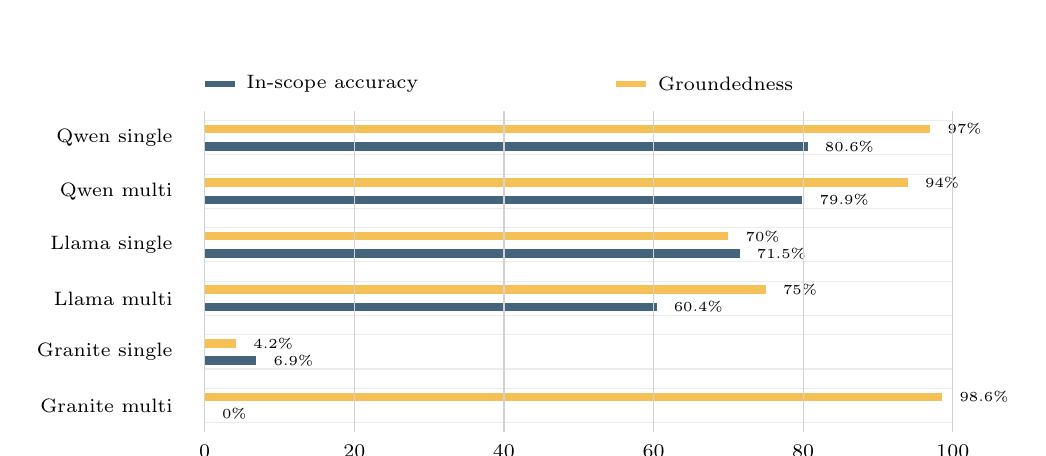
\begin{tikzpicture}[x=0.095cm,y=0.68cm]
  \foreach \y/\name/\a/\g in {6/Qwen single/80.6/97,5/Qwen multi/79.9/94,4/Llama single/71.5/70,3/Llama multi/60.4/75,2/Granite single/6.9/4.2,1/Granite multi/0/98.6} {
    \node[anchor=east,font=\scriptsize] at (-3,\y) {\name};
    \draw[gray!15] (0,\y-0.32) rectangle (100,\y+0.32);
    \fill[iitblue!80] (0,\y-0.24) rectangle (\a,\y-0.08);
    \fill[iitgold!90] (0,\y+0.08) rectangle (\g,\y+0.24);
    \node[anchor=west,font=\tiny] at (\a+1,\y-0.16) {\a\%};
    \node[anchor=west,font=\tiny] at (\g+1,\y+0.16) {\g\%};
  }
  \foreach \x in {0,20,40,60,80,100} {\draw[gray!35] (\x,0.5) -- (\x,6.5); \node[font=\scriptsize,anchor=north] at (\x,0.45) {\x};}
  \draw[iitblue!80,line width=2pt] (0,7) -- (4,7) node[right,font=\scriptsize,black]{In-scope accuracy};
  \draw[iitgold!90,line width=2pt] (55,7) -- (59,7) node[right,font=\scriptsize,black]{Groundedness};
\end{tikzpicture}
\caption{In-scope accuracy and groundedness. Granite multi groundedness is high only because pseudo-tool text contains few factual claims; it does not indicate useful answers.}
\label{fig:main-bars}
\end{figure}

\begin{figure}[H]
\centering
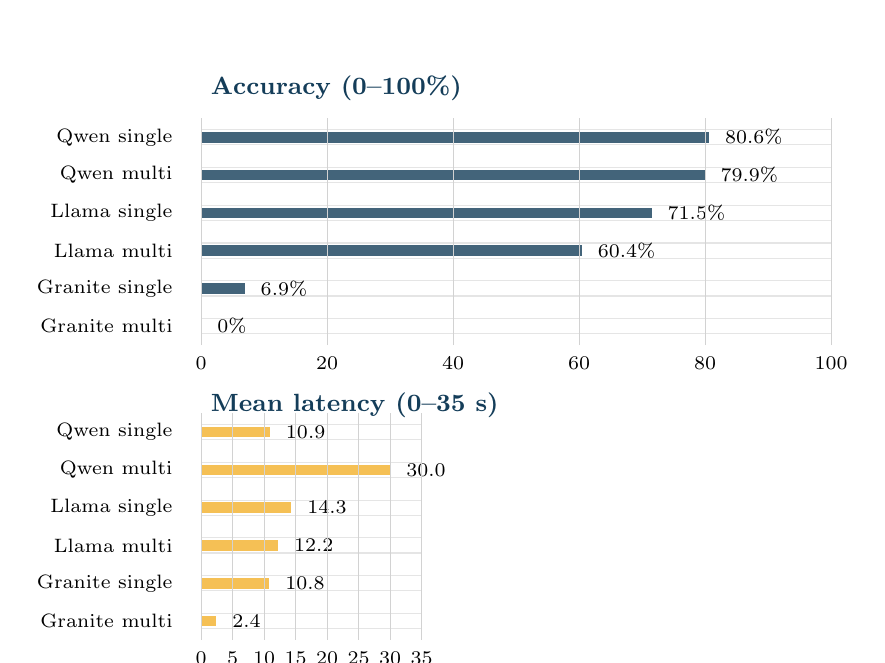
\begin{tikzpicture}[x=0.08cm,y=0.48cm]
  \node[anchor=west,font=\small\bfseries,color=iitblue] at (0,7.3) {Accuracy (0--100\%)};
  \node[anchor=west,font=\small\bfseries,color=iitblue] at (0,-1.1) {Mean latency (0--35 s)};
  \foreach \y/\name/\acc/\lat in {6/Qwen single/80.6/10.9,5/Qwen multi/79.9/30.0,4/Llama single/71.5/14.3,3/Llama multi/60.4/12.2,2/Granite single/6.9/10.8,1/Granite multi/0/2.4} {
    \node[anchor=east,font=\scriptsize] at (-3,\y) {\name};
    \draw[gray!20] (0,\y-0.20) rectangle (100,\y+0.20);
    \fill[iitblue!80] (0,\y-0.14) rectangle (\acc,\y+0.14);
    \node[anchor=west,font=\scriptsize] at (\acc+1,\y) {\acc\%};
    \node[anchor=east,font=\scriptsize] at (-3,{\y-7.8}) {\name};
    \draw[gray!20] (0,{\y-7.8-0.20}) rectangle (35,{\y-7.8+0.20});
    \fill[iitgold!90] (0,{\y-7.8-0.14}) rectangle (\lat,{\y-7.8+0.14});
    \node[anchor=west,font=\scriptsize] at (\lat+1,{\y-7.8}) {\lat};
  }
  \foreach \x in {0,20,40,60,80,100} {\draw[gray!35] (\x,0.5) -- (\x,6.5); \node[font=\scriptsize,anchor=north] at (\x,0.45) {\x};}
  \foreach \x in {0,5,10,15,20,25,30,35} {\draw[gray!35] (\x,-7.3) -- (\x,-1.3); \node[font=\scriptsize,anchor=north] at (\x,-7.35) {\x};}
\end{tikzpicture}
\caption{Accuracy and mean response latency on separate scales.}
\label{fig:quality-latency}
\end{figure}

\subsection{Accuracy by question category}
\begin{table}[H]
\centering
\caption{Accuracy by category (percent).}
\label{tab:category}
\small
\begin{tabular}{llrrrr}
\toprule
\textbf{Model} & \textbf{Mode} & \textbf{Policy} & \textbf{Schedule} & \textbf{Email} & \textbf{Out of scope}\\
\midrule
Qwen3:8b & Single & 67 & 100 & 83 & 100\\
Qwen3:8b & Multi & 81 & 98 & 42 & 100\\
Qwen3:8b & Multi, no think & 68 & 98 & 38 & 100\\
Llama3.1:8b & Single & 68 & 98 & 29 & 100\\
Llama3.1:8b & Multi & 62 & 83 & 8 & 100\\
Granite3.3:8b & Single & 6 & 8 & 8 & 94\\
Granite3.3:8b & Multi & 0 & 0 & 0 & 89\\
\bottomrule
\end{tabular}
\end{table}

\begin{figure}[H]
\centering
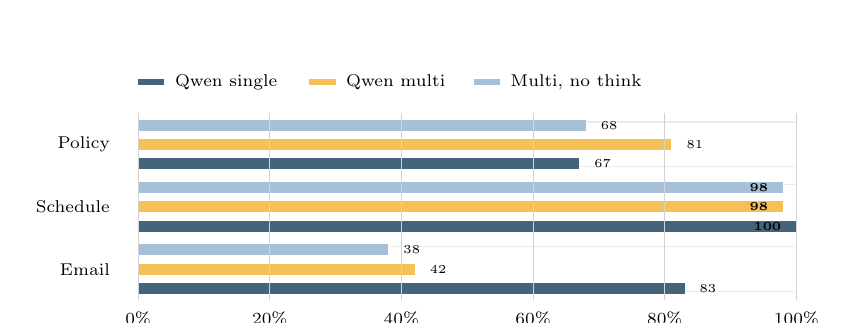
\begin{tikzpicture}[scale=0.88,transform shape,x=0.095cm,y=0.90cm]
  \foreach \y/\name/\a/\b/\c in {6/Policy/67/81/68,5/Schedule/100/98/98,4/Email/83/42/38} {
    \node[anchor=east,font=\scriptsize] at (-3,\y) {\name};
    \draw[gray!15] (0,\y-0.36) rectangle (100,\y+0.36);
    \fill[iitblue!80] (0,\y-0.40) rectangle (\a,\y-0.22);
    \fill[iitgold!90] (0,\y-0.09) rectangle (\b,\y+0.09);
    \fill[midblue!45] (0,\y+0.22) rectangle (\c,\y+0.40);
    \ifnum\a>90 \node[anchor=east,font=\tiny\bfseries] at ({\a-1},\y-0.31) {\a}; \else \node[anchor=west,font=\tiny] at (\a+1,\y-0.31) {\a}; \fi
    \ifnum\b>90 \node[anchor=east,font=\tiny\bfseries] at ({\b-1},\y) {\b}; \else \node[anchor=west,font=\tiny] at (\b+1,\y) {\b}; \fi
    \ifnum\c>90 \node[anchor=east,font=\tiny\bfseries] at ({\c-1},\y+0.31) {\c}; \else \node[anchor=west,font=\tiny] at (\c+1,\y+0.31) {\c}; \fi
  }
  \foreach \x in {0,20,40,60,80,100} {\draw[gray!35] (\x,3.5) -- (\x,6.5); \node[font=\scriptsize,anchor=north] at (\x,3.45) {\x\%};}
  \draw[iitblue!80,line width=2pt] (0,7) -- (4,7) node[right,font=\scriptsize,black]{Qwen single};
  \draw[iitgold!90,line width=2pt] (26,7) -- (30,7) node[right,font=\scriptsize,black]{Qwen multi};
  \draw[midblue!45,line width=2pt] (51,7) -- (55,7) node[right,font=\scriptsize,black]{Multi, no think};
\end{tikzpicture}
\caption{Qwen3 category-wise comparison. Specialisation improves policy accuracy but reduces email accuracy in this implementation.}
\label{fig:qwen-category}
\end{figure}

\subsection{Deterministic checks}
\begin{table}[H]
\centering
\caption{Deterministic tool and retrieval checks (percent, except counts).}
\label{tab:deterministic}
\small
\begin{tabular}{llrrrr}
\toprule
\textbf{Model} & \textbf{Mode} & \textbf{Cites returned source} & \textbf{Gold source} & \textbf{Empty} & \textbf{Errors}\\
\midrule
Qwen3:8b & Single & 85 & 89 & 0 & 0\\
Qwen3:8b & Multi & 100 & 90 & 0 & 0\\
Qwen3:8b & Multi, no think & 95 & 83 & 6 & 0\\
Llama3.1:8b & Single & 98 & 94 & 0 & 0\\
Llama3.1:8b & Multi & 95 & 86 & 0 & 0\\
Granite3.3:8b & Single & 2 & 8 & 0 & 0\\
Granite3.3:8b & Multi & 0 & 0 & 0 & 0\\
\bottomrule
\end{tabular}
\end{table}

\section{Analysis of Findings}
\label{sec:findings}

\subsection{Qwen3 is the strongest practical choice}
Qwen3:8b is the only model that combines high answer quality, strong grounding and perfect refusal behavior in both modes. The single agent has the best measured accuracy and substantially lower latency. The multi-agent version has slightly lower accuracy but improves citation correctness from 80\% to 90\%, routing accuracy to 96.7\% and run consistency to 86.7\%. Thus, the multi-agent design is justified when modularity, observability and specialist separation are priorities, while the single agent is the better latency-sensitive deployment.

\subsection{Specialisation is not automatically beneficial}
The multi-agent version improves Qwen3's policy performance from 67\% to 81\%, likely because the policy specialist has a narrower prompt and a focused tool set. The same decomposition hurts Llama3.1:8b, whose accuracy falls from 71.5\% to 60.4\%. An additional transfer creates another opportunity for malformed arguments, premature refusal or failure to continue after routing.

\subsection{Thinking in the orchestrator fixes silent routing failures}
With Qwen3's orchestrator thinking disabled, two ambiguous questions repeatedly returned empty messages. Enabling thinking only for the orchestrator reduced empty answers from six to zero, increased routing accuracy from 90\% to 96.7\% and increased in-scope accuracy from 72.9\% to 79.9\%. The cost was mean latency increasing from 13.0\,s to 30.0\,s and p90 latency increasing from 23.0\,s to 53.5\,s.

\subsection{Out-of-scope refusal and logging are strong}
Qwen3 and Llama3.1 refused 100\% of out-of-scope questions and logged them 100\% of the time. The callback was essential: Qwen3 frequently produced the refusal but did not call \tool{log\_unanswered} itself, so the callback provided the safety guarantee. False refusals remain a concern, ranging from 3\% to 12\% for Qwen3 and Llama3.1.

\subsection{Granite is unsuitable for this tool-calling design}
Granite3.3:8b did not reliably emit structured tool calls through the Ollama configuration. In multi-agent mode it often printed a pseudo transfer instruction as the answer. Its apparent 98.6\% groundedness is therefore not evidence of useful performance: the output often contained no factual claim at all. A one-tool probe should be mandatory before replacing the selected model.

\section{Failure Modes and Limitations}
\label{sec:limitations}

\begin{enumerate}[leftmargin=*]
  \item \textbf{Email ambiguity:} Questions asking both for procedural policy and an email can be routed to the wrong specialist. Qwen3 multi-agent email accuracy is only 42\%, compared with 83\% for the single agent.
  \item \textbf{Superseded regulations:} The July 2024 attendance and examination circulars supersede older rules. Models sometimes combine the old and new policy instead of explicitly preferring the amendment.
  \item \textbf{Synthetic structured fields:} Some course codes, room assignments and course-to-instructor mappings are illustrative. The report and UI must label these fields clearly.
  \item \textbf{Small evaluation set:} The experiment contains only 30 questions and three repeated runs. Differences of a few percentage points may reflect sampling noise.
  \item \textbf{Latency:} A thinking orchestrator adds nearly three times the mean latency of Qwen3 single-agent mode. This may be unacceptable for interactive use without streaming or caching.
  \item \textbf{External judge dependency:} The evaluation judge uses Claude Sonnet 5.5. The judge itself can introduce subjectivity, especially for partial answers and citation quality.
\end{enumerate}

\section{Recommendations and Future Work}
\label{sec:future}

\begin{enumerate}[leftmargin=*]
  \item Deploy Qwen3:8b single-agent mode where latency is the primary objective; deploy multi-agent mode where specialist modularity and routing telemetry are more important.
  \item Require the exact course name when an email query does not contain a course code, and make \tool{not\_found} responses suggest retrying with the title.
  \item Add document dates and explicit ``superseded by'' metadata to retrieval chunks, with a ranking boost for newer circulars.
  \item Reject any user-facing statement that a draft was saved unless the runner has a corresponding successful \tool{draft\_email} event.
  \item Expand the question set with paraphrases, multilingual queries, adversarial near-misses and more conflicts between old and new regulations.
  \item Add retrieval confidence, source freshness and tool traces to the evaluation dashboard.
  \item Use a structured output schema for every specialist and validate the schema before returning an answer.
  \item Add a human review workflow for unanswered questions and resolved staff responses, allowing the corpus to improve over time.
\end{enumerate}

\section{Reproducibility}
\label{sec:reproducibility}

The repository contains the source code, data manifest, structured data, question set, raw evaluation runs, judge verdicts and scoring scripts. A fresh setup is:

\begin{lstlisting}[language=bash]
uv sync --python 3.12
cp .env.example .env
uv run python scripts/fetch_docs.py
uv run python scripts/ocr_scans.py
uv run pytest -q
uv run python -m helpdesk.ingest
uv run python scripts/check_retrieval.py
uv run python eval/run_eval.py
uv run python eval/judge.py
uv run python eval/score.py
\end{lstlisting}

The interactive modes are:

\begin{lstlisting}[language=bash]
uv run python -m helpdesk.cli "What is the slot for the course Autonomous Systems?"
uv run python -m helpdesk.cli --mode multi
uv run streamlit run app/streamlit_app.py
\end{lstlisting}

\section{Conclusion}
\label{sec:conclusion}

This project demonstrates a practical pattern for a bounded institutional assistant. The combination of retrieval, structured tools, specialist agents, citations, refusal logging and directory validation is more reliable than unconstrained generation. The evaluation confirms that Qwen3:8b is the most suitable tested model for the current tool-calling stack. The single-agent configuration is the best baseline for accuracy and latency, while the multi-agent configuration provides better modularity, routing visibility and citation behavior at a substantial latency cost. The most important engineering lesson is that deterministic safeguards must remain outside the language model: callbacks must log refusals, tools must validate recipients, and the runner must verify that claimed actions actually occurred.

\appendix
\section{Evaluation Question Categories}
\label{app:questions}

\begin{longtable}{>{\raggedright\arraybackslash}p{0.12\textwidth} >{\raggedright\arraybackslash}p{0.77\textwidth}}
\caption{Question identifiers and examples from the evaluation set.}\\
\toprule
\textbf{ID} & \textbf{Question}\\
\midrule
\endfirsthead
\toprule
\textbf{ID} & \textbf{Question}\\
\midrule
\endhead
P01 & What is the attendance requirement to sit in the Major exam?\\
P02 & How many Open Elective credits do I need to earn in order to get a B.Tech. Degree?\\
P03 & I missed my Major exam because I was ill. How do I apply for a make-up exam?\\
P04 & When are the Major examinations for Semester I of 2026--27?\\
P05 & How long is the Major examination and what is its minimum weightage?\\
P06 & What happens if I am absent from all academic activities for four weeks in a semester?\\
P07 & What is the last date to add or drop courses in Semester I 2026--27?\\
P08 & To whom should a B.Tech. student address an application for leave of absence?\\
P09 & How many total credits are required for a regular B.Tech. degree?\\
P10 & How many credits must a B.Tech. student earn by the end of the second semester?\\
P11 & When is the Minor examination in Semester I 2026--27?\\
P12 & What is the maximum duration allowed to complete a B.Tech. programme?\\
S01 & What is the slot for the course Autonomous Systems?\\
S02 & How many 400-level electives have been floated by the Humanities department?\\
S03 & What classes do I have on Friday?\\
S04 & Which room is Computational Game Theory held in?\\
S05 & On which days and at what time does slot F meet?\\
S06 & How many 700-level electives is the Computer Science department offering?\\
S07 & How many credits is Environmental Science and what is its L-T-P structure?\\
S08 & When is CSL7570 scheduled?\\
E01--E04 & Instructor contact and email-drafting requests, including leave and make-up exam emails.\\
O01--O06 & Out-of-scope questions about dining, campus travel, facilities, current officials and placement statistics.\\
\bottomrule
\end{longtable}

\section{References}
\sloppy
\begin{enumerate}[leftmargin=*]
  \item IIT Jodhpur academic regulations, curricula, examination circulars and academic calendars collected in \texttt{data/raw/}.
  \item Academic Helpdesk Agent repository, \url{https://github.com/Mohi1038/academic-helpdesk-agent}.
  \item Google Agent Development Kit documentation, \url{https://google.github.io/adk-docs/}.
  \item ChromaDB documentation, \url{https://docs.trychroma.com/}.
  \item Ollama documentation, \url{https://ollama.com/}.
\end{enumerate}

\end{document}
